
\def\QS{15}
\def\s{1.5}
\def\lw{0.4}

\tikzset{
  qubit/.style={line width=\lw,circle,draw,fill=white,minimum size=\QS},
  bound/.style={line width=\lw,circle, fill=gray!50, minimum size=\QS},
  line/.style={line width=\lw},
  xer/.style={line width=\lw,circle,draw,fill=red!50,inner sep=0,text width=\QS,align=center},
  zer/.style={line width=\lw,circle,draw,fill=cyan!50,inner sep=0,text width=\QS,align=center},
  yer/.style={line width=\lw,circle,draw,fill=orange!50,inner sep=0,text width=\QS,align=center},
  plaq/.style={fill=cyan!20},
  vert/.style={red!50, line width=4*\lw},
  synz/.style={cyan!50, line width=4*\lw, line cap=round},
  synx/.style={purple!25, line width=4*\lw, line cap=round},
  empty/.style={inner sep=0},
  arrow/.style={->, line width=2*\lw},
  script/.style={rectangle, fill=white, opacity=.5, text opacity=1, inner sep=0}
  }

\pgfdeclarelayer{bg}
\pgfdeclarelayer{edges}
\pgfdeclarelayer{qubits}
\pgfsetlayers{bg,edges,qubits,main}

\newcommand{\MINUS}[1]{%
  \number\numexpr#1-1\relax%
}


\newcommand\DRAWTORIC[1]{
  % Draws a toric lattice
  % var 0:    lattice size

  \def\LS{\MINUS{#1}}
  \begin{pgfonlayer}{edges}
    \foreach \x in {0,...,\LS}{
      \draw[line width=\lw] (0,\s*\x) -- (\s*\LS+\s,\s*\x) (\s*\x, -\s) -- (\s*\x, \s*\LS);
      \draw[line width=\lw, dotted] (0,\s*\x - \s/2) -- (\s*\LS+\s,\s*\x - \s/2) (\s*\x + \s/2, -\s) -- (\s*\x + \s/2, \s*\LS);
      }
    \draw[line width=\lw, dashed] (0, -\s) -- (\s*\LS+\s, -\s) -- (\s*\LS+\s, \s*\LS);
  \end{pgfonlayer}
  \begin{pgfonlayer}{qubits}
    \foreach \x in {0,...,\LS}
      \foreach \y in {0,...,\LS}{
         \node [qubit] (N-\x-\y-0) at (\s*\x + \s/2, \s*\y) {};
         \node [qubit] (N-\x-\y-1) at (\s*\x, \s*\y - \s/2) {};
         \coordinate (P-\x-\y) at (\s*\x + \s/2, \s*\y - \s/2);
         \coordinate (S-\x-\y) at (\s*\x, \s*\y);
         }
    \foreach \x in {0,...,\LS}{
      \node [bound] (By-\x) at (\s*\LS+\s, \s*\x - \s/2) {};
      \node [bound] (Bx-\x) at (\s*\x + \s/2, -\s) {};
      \coordinate (S-\x-#1) at (\s*\x, -\s);
      \coordinate (S-#1-\x) at (\s*#1, \s*\x);
    }

  \end{pgfonlayer}
}

\newcommand\DRAWPLANAR[1]{
  % Draws a planar lattice#1
  % var 0:    lattice size

  \def\LS{\MINUS{#1}}
  \begin{pgfonlayer}{edges}
    \foreach \x in {1,...,\LS}{
      \draw (\s/2,\s*\x) -- (\s*\LS+\s/2,\s*\x) (\s*\x, 0) -- (\s*\x, \s*\LS);
      \draw[dotted] (\s*\x + \s/2, 0) -- (\s*\x + \s/2, \s*\LS) (\s/2,\s*\x - \s/2) -- (\s*\LS+\s/2,\s*\x - \s/2);
      }
    \draw (\s/2,0) -- (\s*\LS+\s/2,0);
    \draw[dotted] (\s/2, 0) -- (\s/2, \s*\LS);
  \end{pgfonlayer}
  \begin{pgfonlayer}{qubits}
    \foreach \x in {1,...,\LS}
      \foreach \y in {1,...,\LS}{
         \node [qubit] (N-\x-\y-0) at (\s*\x + \s/2, \s*\y) {};
         \node [qubit] (N-\x-\y-1) at (\s*\x, \s*\y - \s/2) {};
         \coordinate (P-\x-\y) at (\s*\x + \s/2, \s*\y - \s/2);
         \coordinate (S-\x-\y) at (\s*\x, \s*\y);
         }
    \foreach \x in {0,...,\LS}{
      \node [qubit] (N-\x-0-0) at (\s*\x + \s/2, 0) {};
      \node [qubit] (N-0-\x-0) at (\s/2, \s*\x) {};
      \coordinate (P-0-\x) at (\s/2, \s*\x - \s/2);
      \coordinate (S-\x-0) at (\s*\x, 0);
    }
  \end{pgfonlayer}
}


\newcommand\DRAWERROR[4]{
  % Draws a toric lattice
  % var 0:    y coordinate
  % var 1:    x coordinate
  % var 2:    td coordinate
  % var 3:    error type x,y,z
  \def\x{#1}
  \def\y{#2}
  \begin{pgfonlayer}{qubits}    % select the background layer
    \ifstrequal{#4}{x}%
      {\ifnumequal{#3}{0}
        {\node [xer] (\y,\x,0) at (\s*\x + \s/2, \s*\y) {\tiny X};}
        {\node [xer] (\y,\x,0) at (\s*\x, \s*\y - \s/2) {\tiny X};}}
      {}
    \ifstrequal{#4}{z}%
      {\ifnumequal{#3}{0}
        {\node [zer] (\y,\x,0) at (\s*\x + \s/2, \s*\y) {\tiny Z};}
        {\node [zer] (\y,\x,0) at (\s*\x, \s*\y - \s/2) {\tiny Z};}}
      {}
    \ifstrequal{#4}{y}%
      {\ifnumequal{#3}{0}
        {\node [yer] (\y,\x,0) at (\s*\x + \s/2, \s*\y) {\tiny Y};}
        {\node [yer] (\y,\x,0) at (\s*\x, \s*\y - \s/2) {\tiny Y};}}
      {}
  \end{pgfonlayer}
}

\newcommand\DRAWPLAQ[2]{
  % Draws a plaquette
  % var 0:    y coordinate
  % var 1:    x coordinate
  \def\x{#1}
  \def\y{#2}
  \begin{pgfonlayer}{bg}
    \fill[plaq] (\x*\s,\y*\s) rectangle (\x*\s+\s,\y*\s-\s);
  \end{pgfonlayer}
}

\newcommand\DRAWEPLAQ[2]{
  % Draws a plaquette
  % var 1:    x coordinate
  % var 2:    y coordinate
  \def\x{#1}
  \def\y{#2}
  \begin{pgfonlayer}{bg}
    \ifnumequal{\x}{0}
      {\fill[plaq] (.5*\s,\y*\s) rectangle (\s,\y*\s-\s);}
      {\fill[plaq] (\x*\s,\y*\s) rectangle (\x*\s + .5*\s,\y*\s-\s);}
  \end{pgfonlayer}
}

\newcommand\DRAWSTAR[3]{
  % Draws a star
  % var 0:    y coordinate
  % var 1:    x coordinate
  % var 2:    lattice size
  \def\x{#1}
  \def\y{#2}
  \begin{pgfonlayer}{edges}
    \ifnumequal{\x}{0}
      {\draw[vert] (#3*\s-\s/2, \y*\s) -- (#3*\s, \y*\s);}
      {\draw[vert] (\x*\s-\s/2, \y*\s) -- (\x*\s, \y*\s);}
    \ifnumequal{\y}{\LS}
      {\draw[vert] (\x*\s, -\s) -- (\x*\s, -\s/2);}
      {\draw[vert] (\x*\s, \y*\s) -- (\x*\s, \y*\s +\s/2);}
    \draw[vert] (\x*\s, \y*\s - \s/2) -- (\x*\s, \y*\s) -- (\x*\s + \s/2, \y*\s);
  \end{pgfonlayer}
}


\newcommand\DRAWESTAR[2]{
  % Draws a star
  % var 1:    x coordinate
  % var 2:    y coordinate
  \def\x{#1}
  \def\y{#2}
  \begin{pgfonlayer}{edges}
    \ifnumequal{\y}{0}
      {\draw[vert] (\x*\s, 0) -- (\x*\s, \s/2);}
      {\draw[vert] (\x*\s, \y*\s) -- (\x*\s, \y*\s-\s/2);}
    \draw[vert] (\x*\s - \s/2, \y*\s) -- (\x*\s + \s/2, \y*\s);
  \end{pgfonlayer}
}



\newcommand\DSPECTRUM[3]{
  \tikzmath{
    \size = #1;
    \X = #2;
    \Y = #3;
    \y = #3-0.1;
  }
  \ifnumequal{\X}{0}{}{
    \path[fill=white!50!black, rounded corners=1pt] (0, 0.1) rectangle (\X,\y);
  }
  \draw[line width =0.5] (0,\Y) -- (0,0) -- (\size,0) -- (\size,\Y);

  \foreach \xx in {0,...,\size}{
    \draw[line width=0.5, font=\footnotesize] (\xx,0) -- +(0,-0.1) node[below] {\xx};
  }
}

\newcommand\DSPECTRA[6]{
  \tikzmath{
    \M = #1;
    \I = #2;
    \x = #3;
    \y = #4;
    \h = #5;
    \w = #6;
    \X = \x + \M;
  }
  \begin{scope}[shift={(\x, 0)}]
  \begin{scope}[xscale=\w]
  
  \ifnumequal{\I}{0}{}{
    \draw[line width=0, fill=white!50!black, rounded corners=2pt] (0,\y) rectangle +(\I,\h);
  }
  \draw[thin, rounded corners = 2pt] (0,\y) rectangle +(\M,\h);
  \foreach [count=\i] \xx in {0,...,\M}{
    \draw[font=\tiny] (\xx,\y) node[below] {\xx};
  }
  \end{scope}
  \end{scope}
}

\chapter{The surface code}

\begin{figure}[h]
  \centering
  \begin{tikzpicture}
    \DRAWTORIC{3}
    \draw [arrow] (-1,0 |- N-0-2-1) node [align=right, left] {qubit/edge} -- (N-0-2-1);
    \node (plaquette) at ($(N-0-1-0)!0.5!(N-0-0-0)$) {};
    \node (star) at ($(N-1-0-1)!0.5!(N-1-1-1)$) {};
    \draw [arrow] (-1,0 |- plaquette)  node [align=right, left] {face} -- (plaquette);
    \draw [arrow] (-1,0 |- N-1-0-1) node [align=right, left] {vertex} to [out=0, in=225] (star);
    \node [align=left, right] at (3*\s + .5, .5*\s) {periodic boundary};

  \end{tikzpicture}
  \caption{The toric code is defined as a $L\times L$ lattice (here $L=3$) with periodic boundary conditions. The edges on the lattice, which represents the qubits, make up faces and vertices.}\label{fig:sf_toriclattice}
\end{figure}

The variant of the stabilizer codes that we are going to explore in this thesis is Kitaev's \emph{surface code}, which is of the category of \emph{topological codes}. Among this category, the surface code is preferable as it offers the highest error tolerance under realise noise channels and requires only local stabilizer measurements of physically neighboring qubits. Two variants of the surface code will be considered here, the \emph{toric code} in section \ref{sec:surface_toric} and the \emph{planar code} in section \ref{sec:surface_planar}. The various error channels our code will undergo is explained in section \ref{sec:surface_error}, and various decoders are detailed in \ref{sec:surface_decoders}.


\section{The toric code}\label{sec:surface_toric}

The \emph{toric code} is defined by arranging qubits on the edges of a square lattice with periodic boundary conditions, as seen in Figure \ref{fig:sf_toriclattice}. The name of the toric code lends itself from the torus, or donut, shape, where any point on the surface of the torus will encounter itself after traversing the torus in either x or y directions. Hence, the top edge of the toric code meets the bottom edge, whereas the left edge meets the right. On a $L\times L$ grid there are $N = 2L^2$ edges and the same amount of physical qubits. This topology of qubit arrangement plays an important part in encoding the logical qubits, which is stored in the non-trivial cycles on the torus. Errors, beneath a certain threshold, will only introduce local effects and does not change these cycles.

\subsection{Stabilizer generators}

To define a stabilizer code, we need to specify the $m$ independent stabilizer generators and the encoded $\bar{X}$ and $\bar{Z}$ operators. On the toric code there are two types of stabilizer generators, \emph{plaquette} and \emph{star} operators, which are associated with the \emph{faces} and \emph{vertices} of the square lattice, respectively.

\begin{figure}
  \centering
  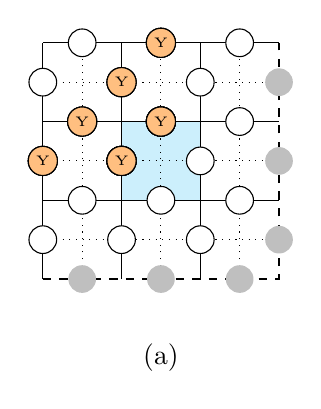
\begin{tikzpicture}
    \DRAWTORIC{3}
    \DRAWPLAQ{1}{1}
    \DRAWERROR{1}{1}{0}{z}
    \DRAWERROR{1}{1}{1}{z}
    \DRAWERROR{0}{1}{0}{z}
    \DRAWERROR{1}{2}{1}{z}
    \node[below of=Bx-1] {(a)};
  \end{tikzpicture}
  \hspace{1cm}
  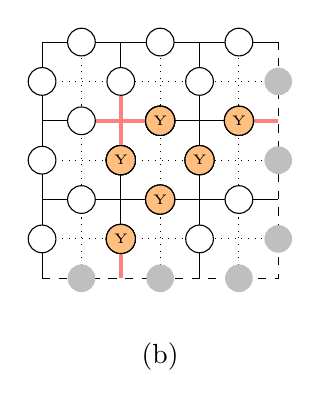
\begin{tikzpicture}
    \DRAWTORIC{3}
    \DRAWSTAR{1}{1}{3}
    \DRAWERROR{1}{1}{1}{x}
    \DRAWERROR{1}{1}{0}{x}
    \DRAWERROR{2}{1}{1}{x}
    \DRAWERROR{1}{0}{0}{x}
    \node[below of=Bx-1] {(b)};
  \end{tikzpicture}
  \caption{Each face (a) and vertex (b) on the lattice represents a plaquette and star operator, respectively. The non-identity single qubit operators on which they act are indicated. The set of all (but one) plaquettes and vertices make up the stabilizers of the code. }\label{fig:sf_stabilizers}
\end{figure}

\paragraph{Plaquette operators}
For every face $f$ on our lattice, we define a plaquette operator $P_f$, consisting of tensor product of Pauli Z operators on qubits on these edges (see Figure \ref{fig:sf_toriclattice}a),
\begin{equation}\label{eq:sf_plaquette}
  P_f = \bigotimes_{i\in Q(f)} Z_i
\end{equation}
where $Q(f)$ is the set of qubits touching face $f$. On a $L\times L$ grid there are $L^2$ plaquettes.

\paragraph{Star operators}

Similarly, for every vertex $v$ on our lattice, we define a star operator $S_v$, consisting of tensor product of Pauli X operators on qubits neighboring the vertex (see Figure \ref{fig:sf_toriclattice}b),
\begin{equation}\label{eq:sf_plaquette}
  S_v = \bigotimes_{i\in Q(v)} X_i
\end{equation}
where $Q(v)$ is the set of qubits neighboring vertex $v$. On a $L\times L$ grid there are $L^2$ plaquettes.

The full stabilizer of the code can be generated by multiplying elements of the generator operators. Consider two plaquette operators. These two operators will either share one boundary consisting of a qubit, or none. This means that the Pauli Z operator on the boundary qubit will add up to identity as they commute. The result is that the product of the plaquette operators will consists of the overall boundary Pauli operators of the joint plaquette (see Figure \ref{fig:sf_multistab}a).

However, if all plaquettes are applied to the lattice, no boundary will be left. Thus the product of all plaquettes is the identity, which means that the full set of plaquettes are not independent. The full set of stabilizer generators can therefore be completed by simply removing a single plaquette from all available plaquettes. There are therefore $L^2 - 1$ independent plaquette operators. 

The multiplication of star operators follow the same properties as the plaquette operators described above (see Figure \ref{fig:sf_multistab}b). Thus there are also $L^2 - 1$ independent star operators, which sum up to $N_S = 2L^2 - 2$ independent stabilizers. 

\begin{figure}
  \centering
  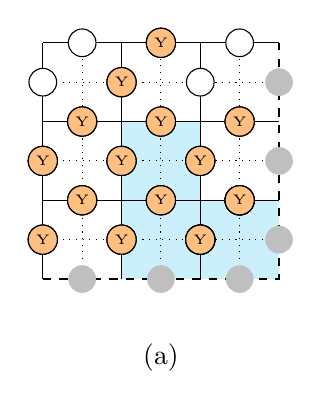
\begin{tikzpicture}
    \DRAWTORIC{3}
    \DRAWPLAQ{1}{1}
    \DRAWPLAQ{1}{0}
    \DRAWPLAQ{2}{0}
    \DRAWERROR{1}{1}{0}{z}
    \DRAWERROR{0}{1}{0}{z}
    \DRAWERROR{1}{2}{1}{z}
    \DRAWERROR{0}{0}{0}{z}
    \DRAWERROR{1}{0}{1}{z}
    \DRAWERROR{2}{0}{1}{z}
    \DRAWERROR{2}{0}{0}{z}
    \DRAWERROR{2}{1}{1}{z}
    \node[below of=Bx-1] {(a)};
  \end{tikzpicture}
  \hspace{1cm}
  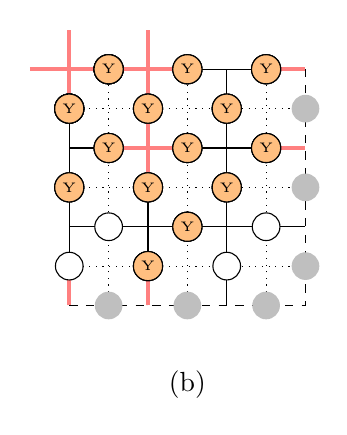
\begin{tikzpicture}
    \DRAWTORIC{3}
    \DRAWSTAR{1}{1}{3}
    \DRAWSTAR{0}{2}{3}
    \DRAWSTAR{1}{2}{3}
    \DRAWERROR{2}{1}{1}{x}
    \DRAWERROR{1}{0}{0}{x}
    \DRAWERROR{2}{2}{1}{x}
    \DRAWERROR{1}{1}{1}{x}
    \DRAWERROR{0}{1}{0}{x}
    \DRAWERROR{0}{2}{1}{x}
    \DRAWERROR{0}{2}{0}{x}
    \DRAWERROR{1}{2}{0}{x}
    \node[below of=Bx-1] {(b)};
  \end{tikzpicture}
  \caption{Each face (a) and vertex (b) on the lattice represents a plaquette and star operator, respectively. The non-identity single qubit operators on which they act are indicated. The set of all (but one) plaquettes and vertices make up the stabilizers of the code. }\label{fig:sf_multistab}
\end{figure}


\subsection{Encoded qubits}
Since there are $N = L^2$ qubits and $N_S = 2L^2 - 2$ independent stabilizers, we must have $N_L = N - N_S = 2$ encoded qubits and therefore 4 logical operators $\bar{X}_1, \bar{X}_2, \bar{Z}_1$ and $\bar{Z}_2$. 

Recall the logical operators consists of the Pauli operators, and must commute with all stabilizer generators, but cannot be part of the stabilizer itself. We can construct the logical operators by starting with, for example, a single Pauli Z operator. It commutes with all plaquette operators trivially. In terms of the star operators, this single Pauli Z operator commutes with all but the two neighboring qubits, as all others apply to different qubits. Adding another Pauli Z operator will shift will of the anticommuting neighboring star operators. We know see that a closed loop of Z operators around the torus does not have neighboring star operators, and therefore commute with all stabilizers. As the torus has two directions we can loop over, these are the logical $\bar{Z}$ operators (see Figure \ref{fig:sf_logical}a). Analogously, we can construct the logical $\bar{X}$ operators in the same way (Figure \ref{fig:sf_logical}b).

\def\QS{10}
\def\s{1}
\begin{figure}
  \centering
  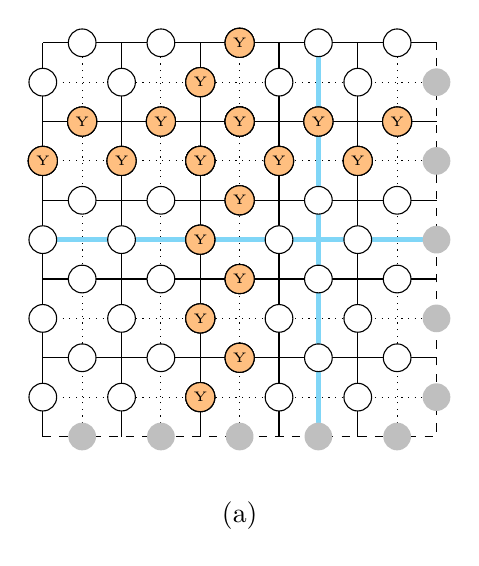
\begin{tikzpicture}
    \DRAWTORIC{5}
    \DRAWERROR{2}{0}{1}{z}
    \DRAWERROR{2}{1}{1}{z}
    \DRAWERROR{2}{2}{1}{z}
    \DRAWERROR{2}{3}{1}{z}
    \DRAWERROR{2}{4}{1}{z}
    \DRAWERROR{0}{3}{0}{z}
    \DRAWERROR{1}{3}{0}{z}
    \DRAWERROR{2}{3}{0}{z}
    \DRAWERROR{3}{3}{0}{z}
    \DRAWERROR{4}{3}{0}{z}
    \begin{pgfonlayer}{edges}
      \draw[synz] (N-0-2-1) -- (By-2);
      \draw[synz] (Bx-3) -- (N-3-4-0);
    \end{pgfonlayer}
    \node[below of=Bx-2] {(a)};
  \end{tikzpicture}
  \hspace{1cm}
  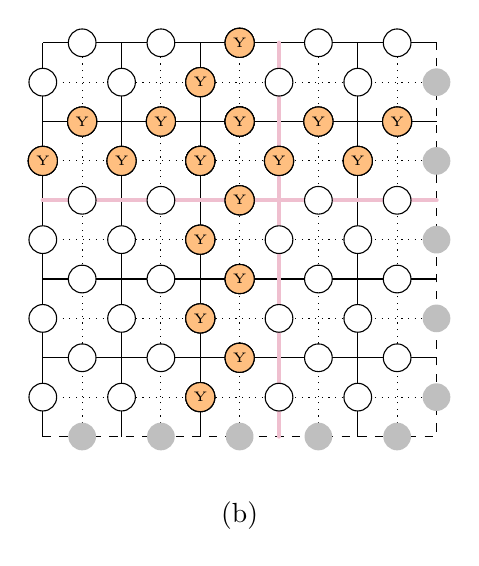
\begin{tikzpicture}
    \DRAWTORIC{5}
    \DRAWERROR{2}{0}{0}{x}
    \DRAWERROR{2}{1}{0}{x}
    \DRAWERROR{2}{2}{0}{x}
    \DRAWERROR{2}{3}{0}{x}
    \DRAWERROR{2}{4}{0}{x}
    \DRAWERROR{0}{3}{1}{x}
    \DRAWERROR{1}{3}{1}{x}
    \DRAWERROR{2}{3}{1}{x}
    \DRAWERROR{3}{3}{1}{x}
    \DRAWERROR{4}{3}{1}{x}
    \begin{pgfonlayer}{edges}
      \draw[synx] (S-0-2) -- (S-0-2 -| 5*\s, 0);
      \draw[synx] (S-3-4) -- (S-3-4 |- 0, -\s);
    \end{pgfonlayer}
    \node[below of=Bx-2] {(b)};
  \end{tikzpicture}
  \caption{Each face (a) and vertex (b) on the lattice represents a plaquette and star operator, respectively. The non-identity single qubit operators on which they act are indicated. The set of all (but one) plaquettes and vertices make up the stabilizers of the code. }\label{fig:sf_logical}
\end{figure}

\subsection{Error detection}
\subsection{Error correction}


\section{Error channels}\label{sec:surface_error}

\section{The planar code}\label{sec:surface_planar}

\begin{figure}
  \centering
  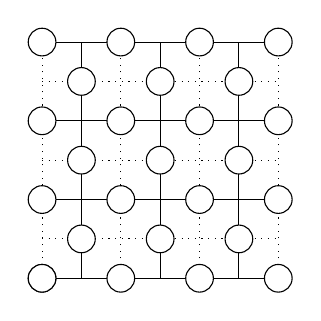
\begin{tikzpicture}
    \DRAWPLANAR{4}
  \end{tikzpicture}
\end{figure}

\section{Decoders}\label{sec:surface_decoders}
\subsection{The optimal decoder}
\subsection{Minimum Weight Perfect Matching}
\subsection{The Union-Find decoder}

Even the fastest MWPM algorithms still have a quadratic time complexity of $\mathcal{O}(n^2\sqrt{n})$, where $n$ is the number of qubits. In order to realistically utilize a decoder with increasing decoding success rates using increasing lattice size, we would need to have a better time complexity. Luckily, an alternative algorithm called the Peeling Decoder has been developed which can solve errors over the erasure channel with a linear time complexity $\mathcal{O}(n)$ \cite{delfosse2017}. The Union-Find Decoder builds on top of the Peeling Decoder to solve for Pauli errors with a time complexity of $\mathcal{O}(n\alpha(n))$, where $\alpha$ is an inverse Ackermann function, which is smaller than 3 for any practical input size \cite{nickerson2017}. However, these algorithms have a tradeoff in the form of a decrease in the error threshold, and has the reported value of $p_{UF} = 9.2\%$.

A topic of interest will be weighted growth function for the Union-find decoder. This function of the algorithm will increase the error threshold to $p_{UF} = 9.9\%$, but has not been fully described in its publication.  In this section, we will describe the original Peeling decoder and the Union-Find decoder.   \\

\subsubsection{The Peeling decoder}
Let $\varepsilon \subset E$ be an erasure, a set of qubits on which an erasure error occurs, and let $\sigma \subset S$ be the measured error syndrome, the subset of stabilizer generators which anticommute with the erasure errors. In the absence of Pauli errors, all errors $P$ must lie inside the erasure. Therefore, for any pair of stabilizer generators in $\sigma$, the path of errors must also be in the erasure, which can be denoted by $P\subset \varepsilon$. Furthermore, due to the fact that errors $P$ are randomly distributed, any coset of errors and stabilizers $P\cdot S$ that solves the error syndrome $\sigma$ is the most likely coset. These features of an erasures forms the basis of the Peeling decoder. In order to find a coset of $P \cdot S$, the decoder reduces the size of the erasure by peeling edges from the erasure, while keeping the syndromes at the new boundary of the erasure. Elements of the syndrome can be moved by applying an correction on the adjacent qubit. At the end, the entire erasure is peeled or removed, and all corrections will have removed the errors up to a stabilizer.

\tikzset{
  anyon/.style={circle, fill=OrangeRed, minimum size=.2cm, inner sep=0},
  erasure/.style={NavyBlue, very thick},
  correction/.style={Green, very thick},
  description/.style={align=#1, anchor=west, text width=4cm},
  description/.default={left},
  error/.style={text=black, pos=0.5}
  }
\tikzset{
  anyon/.style={circle, fill=OrangeRed, minimum size=.2cm, inner sep=0},
  erasure/.style={NavyBlue, very thick},
  correction/.style={Green, very thick},
  description/.style={align=#1, text width=4cm},
  description/.default={left},
  error/.style={text=black, pos=0.5}
  }

\begin{figure}
  \centering
  \begin{tikzpicture}[on grid, scale=0.8]
    \node at (0,4) {a)};
    \draw[step=1cm,gray,thin] (0.1,0.1) grid (3.9,3.9);
    \draw[erasure] (1,1) -- (2,1) node[error]{$X$} -- (3,1) -- (3,2) -- (2,2) -- (1,2) -- cycle node[error]{$X$};
    \draw[erasure] (1,2) -- (1,3) -- (2,3) node[error]{$X$} -- (2,2);
    \node[description={center}] at (2, -.5) {initial state};

    \begin{scope}[shift={(6,0)}]
      \node at (0,4) {b)};
      \draw[step=1cm,gray,thin] (0.1,0.1) grid (3.9,3.9);
      \draw[erasure] (1,1) -- (2,1) node[anyon]{} -- (3,1) -- (3,2) -- (2,2) -- (1,2) node[anyon] (a) {} -- cycle;
      \draw[erasure] (a) -- (1,3) node[anyon]{} -- (2,3) node[anyon]{}-- (2,2);
      \node[description={center}] at (2, -.5) {identify syndrome};
    \end{scope}

    \begin{scope}[shift={(12,-.5)}]
      \draw[thin] (0,4) -- ++(.5,0) ++(.5,0) node[anchor=west]{normal edge};
      \draw[thin] (0,3) -- ++(.5,0) node[error]{$X$} ++(.5,0) node[anchor=west]{Pauli error};
      \draw[erasure] (0,2) -- ++(.5,0) ++(.5,0) node[anchor=west, text=black]{erased edge};
      \draw[thin] (0,1) -- ++(.5,0) node[anyon,pos=.5]{} ++(.5,0) node[anchor=west]{syndrome};
      \draw[correction] (0,0)   -- ++(.5,0) ++(.5,0) node[anchor=west,text=black]{correction edge};
    \end{scope}

    \begin{scope}[shift={(0,-6)}]
      \node at (0,4) {c)};
      \draw[step=1cm,gray,thin] (0.1,0.1) grid (3.9,3.9);
      \draw[erasure] (1,3) node[anyon]{} -- (2,3) node[anyon]{} -- (2,2) -- (1,2) node[anyon]{} -- (1,1) -- (2,1) node[anyon]{} -- (3,1) -- (3,2);
      \node[description={center}] at (2, -.5) {construct $F_{\varepsilon}$};
    \end{scope}

    \begin{scope}[shift={(6,-6)}]
      \node at (0,4) {d)};
      \draw[step=1cm,gray,thin] (0.1,0.1) grid (3.9,3.9);
      \draw[erasure] (1,3) node[anyon]{} -- (2,3) node[anyon]{} -- (2,2) -- (1,2) node[anyon]{} -- (1,1) -- (2,1) node[anyon](a){};
      \draw[erasure, dashed] (a) -- (3,1) node[pos=0, below, text=black]{$v$} node[pos=0.5, above]{$e$} node[pos=1, below, text=black]{$u$};
      \node[description={center}] at (2, -.5) {peel $e=(u,v), u \notin \sigma$};
    \end{scope}

    \begin{scope}[shift={(12,-6)}]
      \node at (0,4) {e)};
      \draw[step=1cm,gray,thin] (0.1,0.1) grid (3.9,3.9);
      \draw[erasure] (1,3) node[anyon]{} -- (2,3) node[anyon]{} -- (2,2) -- (1,2) node[anyon]{} -- (1,1);
      \draw[erasure, dashed] (1,1) node[below, text=black]{$v$} -- (2,1) node[anyon]{} node[pos=0.5, above]{$e$} node[below, text=black]{$u$};
      \node[description={center}] at (2, -.5) {peel $e=(u,v), u \in \sigma$};
    \end{scope}

    \begin{scope}[shift={(0,-12)}]
      \node at (0,4) {f)};
      \draw[step=1cm,gray,thin] (0.1,0.1) grid (3.9,3.9);
      \draw[erasure] (1,3) node[anyon]{} -- (2,3) node[anyon]{} --  (2,2) -- (1,2) node[anyon]{} -- (1,1) node[anyon](a){};
      \draw[correction] (a) node[below, text=black]{$v$} -- (2,1) node[pos=0.5, above]{$e$} node[below, text=black]{$u$};
      \node[description={center}] at (2, -.5) {flip $u,v$, add $e$ to $C$};
    \end{scope}

    \begin{scope}[shift={(6,-12)}]
      \node at (0,4) {g)};
      \draw[step=1cm,gray,thin] (0.1,0.1) grid (3.9,3.9);
      \draw[correction] (1,3) -- (2,3) node[error]{$X$} (2,1) -- (1,1) node[error]{$X$} -- (1,2) node[error]{$X$};
      \node[description={center}] at (2, -.5) {apply correction set $C$};
    \end{scope}

    \begin{scope}[shift={(12,-12)}]
      \node at (0,4) {h)};
      \draw[step=1cm,gray,thin] (0.1,0.1) grid (3.9,3.9);
      \node[description={center}] at (2, -.5) {end state};
    \end{scope}
  \end{tikzpicture}
  \caption{Schematic representation of the Peeling decoder. On an erasure $\m{E}\subset E$ (a), there may be some Pauli errors $P\subset \m{E}$ that anticommutes with some stabilizer measurements (b) that is identified as the syndrome $\sigma$. The first step is to construct a spanning forest $F_\m{E}\subset \m{E}$, a fully connected acyclic graph. Next the decoder sequentially removes leaf edges $e=(u,v)$ from the forest that connect to the forest via only one vertex $v$. If $u\in\sigma$ (e), remove $u$ from $\sigma$, flip $v$ in $\sigma$ and the edge $e$ is added to the correction set $C$ (f). If $u \notin \sigma$, move on the the next leaf. After applying the correction set $C$, all errors on the lattice commutes with the stabilizers, potentially solving the error (h).}
\end{figure}

We will now describe the Peeling decoder as is presented in Algorithm \ref{algo:peel}. In step 1, we will remove all cycles present in $\varepsilon$. We construct a spanning forest $F_\varepsilon$ inside erasure $\varepsilon$, the maximal subsect of edges of $\varepsilon$ that contains no cycles and spans all vertices of $\varepsilon$. From here, we loop over all edges in $F_\varepsilon$ (step 3), starting at a leaf edge $e = \{u,v\}$, removing the leaf edge from $F_\varepsilon$ (step 4), and conditionally add the edge to the correction set $\kappa$ if the pendant vertex $u$ is in $\sigma$ (step 6). If the correction is applied immediately, we can see that the pendant vertex $u$ is removed from $\sigma$ and that the value of $v$ is flipped in $\sigma$. Edges on a branch in the forest will be added to $\kappa$ until $v \in \sigma$, or a generator will be continuously moved from $u$ to $v$ until it encounters another generator, creating a correction path between two syndrome pairs.

\begin{algo}[algotitle=Peeling decoder \cite{delfosse2017}, label=algo:peel]
\begin{algorithm}[H]
    \SetAlgoNoEnd
    \KwData{A graph $G = (V,E)$, an erasure $\varepsilon \subset E$ and syndrome $\sigma \subset V$}
    \KwResult{Correction set $\kappa \subset E$}
    \BlankLine
    construct a spanning forest $F_\varepsilon$ of $\varepsilon$\;
    initialize $\kappa$ by $\kappa = {\O}$\;
    \While{$F_\varepsilon \neq \O$}{
        pick a leaf edge $e = {u,v}$ with pendant vertex $u$, remove $e$ from $F_\varepsilon$ \;
        \If{$u \in \sigma$}{
            add $e$ to $\kappa$, remove $u$ from $\sigma$ and flip $v$ in $\sigma$}
        \Else{do nothing}
    }
    \KwRet{$\kappa$}
\end{algorithm}
\end{algo}

\noindent Note that due the flipping of both $u$ and $v$ in $\sigma$, the parity of the number of generators in $\sigma$ is always preserved. The peeling decoder can therefore always solve erasures with an even parity, as the size of $\sigma$ will drop until at the end the syndrome will be empty $\sigma = \O$, and call errors are corrected up to a stabilizer. This is always the case in the absence of measurement and Pauli errors, as all errors within the erasure either add or remove an even number of generators to or from $\sigma$.

\paragraph{Time complexity of the Peeling decoder}
The spanning forest $F_\varepsilon$ can be constructed in linear time. Also, the loop over the forest can be operated in linear if the list of leaves is pre-computed and updated during the loop. Thus the Peeling decoder has a linear time complexity in the size of the erasure $\mathcal{O}(\abs{\varepsilon})$ and therefore also in the number of qubits $\mathcal{O}(n)$.

\subsubsection{Growing erasures}

Now in the presence of Pauli errors, errors can occur on edges that are now not part of the erasure, and odd parity clusters can occur. Clusters that consists from only a single generator also exist, which are just end-points of syndromes caused by Pauli errors. We must therefore make an erasure $\varepsilon$ from the syndrome $\sigma$ that is compatible with the peeling decoder, which contains only even parity clusters. To do this, we can iteratively grow the clusters with an odd parity by an half-edge on the boundaries on the clusters. When two odd parity clusters meet, the merged cluster will have a even parity, and can now be solved by the peeling decoder.

\paragraph{Union-Find algorithm}

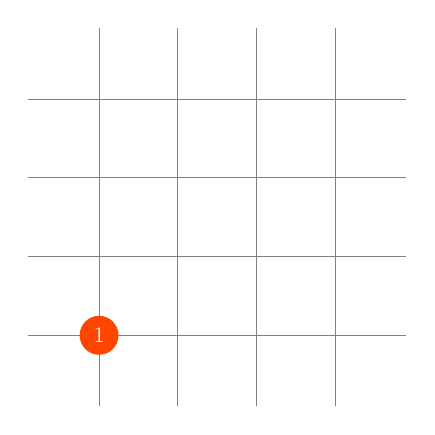
\begin{tikzpicture}
  \draw[step=1cm,gray,thin] (0.1,0.1) grid (4.9, 4.9);
  \node[fill=OrangeRed, circle, text=white, scale=0.8] (N0) at (1, 1) {1};

\end{tikzpicture}

To keep track of the vertices of a cluster, it will be represented as a \emph{cluster tree}, where an arbitrary vertex of the cluster will be the root, and any other vertex will be a child of the root. Whenever an edge $(u,v)$ is fully grown, we will need to traverse the trees of the two vertices $u$ and $v$, and check wether they have the same root; whether they belong to the same cluster. If not, a merge is initiated by making the root of smaller cluster a child of the bigger cluster. These functions, \codefunc{find} and \codefunc{union} respectively, are part of the Union-Find algorithm (not to be confused with the Union-Find decoder) \cite{tarjan}.

\begin{tikzpicture}
  \draw (2,2) circle (0.2);
  \draw (2,2) -- (0,0);)
\end{tikzpicture}

Within the Union-Find algorithm, two features ensure that the complexity of the algorithm is not quadratic. 1). With \textbf{path compression}, as we traverse a tree from child to parent until we reach the root, we make sure that each vertex encountered that we have encountered along the way is pointed directly to the root. This doubles the cost of the \codefunc{find}, but speeds up any future call to any vertex on the traversed path. 2). With \textbf{weighted union}, we make sure to always make the smaller tree a child of the bigger tree. This ensures that the overall length of the path to the root stays minimal. In order to make this happen, we just need to store the size of the tree at the root.

\paragraph{Data structure}
Now it is clear what information is exactly needed to grow the clusters using the Union-Find algorithm. We will need to store the cluster in a sort of cluster-tree. At the root of each tree we store the size and parity of that cluster in order to facilitate weighted union and to select the odd clusters. We will need to store the state of each edge (empty, half-grown, or fully grown) in a table called \codeword{support}. And we need to keep track of the boundary of each cluster in a \codeword{boundary} list.

\paragraph{The routine}
The full routine of the Union-Find decoder as originally described (\cite{nickerson2017}, Algorithm 2) is listed in Algorithm \ref{algo:uf}. In line 1-2, we initialize the data structures, and a list of odd cluster roots $\mathcal{L}$. We will loop over this list until it is empty, or that there are no more odd clusters left.

In each growth iteration, we will need to keep track of which clusters have merged onto one, therefore the fusion list $\mathcal{F}$ is initialized in line 4. We loop over all the edges from the \codeword{boundary} of the clusters from $\mathcal{L}$ in line 5, and grow each edge by an half-edge in \codeword{support}. If an edge is fully grown, it is added to $\mathcal{F}$.

For each edge $(u,v)$ in $\mathcal{F}$, we need to check whether the neighboring vertices belong to different clusters, and merge these clusters if they do. This is done using the Union-Find algorithm in line 6. We call \codefunc{find(u)} and \codefunc{find(v)} to find the cluster roots of the vertices. If they do not have the same root, we make one cluster the child of another by \codefunc{union(u,v)}. Note that this does not only merge two existing clusters, also new vertices, which have themselves as their roots, are added to the cluster this way. We also need to combine the boundary lists of the two clusters.

Finally, we need to update the elements in the cluster list $\mathcal{L}$. First, we replace each element $u$ with its potential new cluster root \codefunc{find(u)} in line 7. We can avoid creating duplicate elements by maintaining an extra look-up table that keeps track of the elements $\mathcal{L}$ at the beginning of each round of growth. In line 8, we update the \codeword{boundary} lists of all the clusters in $\mathcal{L}$, and in line 9, even clusters are removed from the list, preparing it for the next round of growth.

\begin{algo}[algotitle=Union-Find decoder \cite{nickerson2017}, label=algo:uf]
\begin{algorithm}[H]
    \SetAlgoNoEnd
    \KwData{A graph $G = (V,E)$, an erasure $\varepsilon \subset E$ and syndrome $\sigma \subset V$}
    \KwResult{A grown erasure $\varepsilon'$ such that each cluster $\gamma \subset \varepsilon$ is even}
    \BlankLine
    initialize cluster-trees, support and boundary lists for all clusters \;
    initialize list of odd cluster roots $\mathcal{L}$\;
    \While{$\mathcal{L} \neq \emptyset$}{
      initialize fusion list $\mathcal{F}$ \;
      for all $u \in \mathcal{L}$, grow all edges in the boundary list of cluster $C_u$ by a half-edge in support. If the edge is fully grow, add to fusion list $\mathcal{F}$ \;
      for all $e={u,v} \in \mathcal{F}$, if \emph{find($u$)} $\neq$ \emph{find($v$)}, then apply \emph{union($u,v$)}, append boundary list\;
      for all $u \in \mathcal{L}$, replace $u$ with \emph{find($u$)} without creating duplicate elements\;
      for all $u \in \mathcal{L}$, update the boundary list\;
      remove even clusters from $\mathcal{L}$\;
    }
    run peeling decoder with grown erasure $\varepsilon'$
\end{algorithm}
\end{algo}

\subsubsection{Time complexity of the Union-Find decoder}
